\documentclass[letterpaper, 10 pt, conference]{ieeeconf}  % Comment this line out if you need a4paper
%\documentclass[a4paper, 10pt, conference]{ieeeconf}      % Use this line for a4 paper
\IEEEoverridecommandlockouts                              % This command is only needed if 
                                                          % you want to use the \thanks command
\overrideIEEEmargins                                      % Needed to meet printer requirements.

% See the \addtolength command later in the file to balance the column lengths
% on the last page of the document

\usepackage{ieee_packages,graphicx}
\usepackage[left=0.65in,right=0.65in,top=0.7in,bottom=0.7in]{geometry}
\newcommand{\EditTL}[1]{{\color{red}\protect #1}}
%\renewcommand{\EditTL}[1]{{\protect #1}}

\newtheorem{definition}{Definition}
\newtheorem{lem}{Lemma}
\newtheorem{prop}{Proposition}
\newtheorem{cor}{Corollary}
\newtheorem{remark}{Remark}

\title{\LARGE \bf
Geometric Adaptive Control of Attitude Dynamics on $\SO$\\ with State Inequality Constraints}

\author{Shankar Kulumani, Christopher Poole, and Taeyoung Lee
%\thanks{Shankar Kulumani, Christopher Poole, Taeyoung Lee, Mechanical and Aerospace Engineering, George Washington University, Washington DC 20052 {\tt \{skulumani,poolec,tylee\}@gwu.edu}}
%\thanks{This research has been supported in part by NSF under the grants CMMI-1243000, CMMI-1335008, and CNS-1337722.}
}

\begin{document}
\allowdisplaybreaks

\maketitle
\thispagestyle{empty}
\pagestyle{empty}

%%%%%%%%%%%%%%%%%%%%%%%%%%%%%%%%%%%%%%%%%%%%%%%%%%%%%%%%%%%%%%%%%%%%%%%%%%%%%%%%
\section{Motivation}\label{sec:intro}

Rigid body attitude control is an important problem for aerospace vehicles, ground and underwater vehicles, as well as robotic systems~\cite{hughes2004,wertz1978}.
One distinctive feature of the attitude dynamics of rigid bodies is that it evolves on a nonlinear manifold.
The three-dimensional special orthogonal group, or \( \SO \), is the set of \( 3 \times 3 \) orthogonal matrices whose determinant is one.
This configuration space is non-Euclidean and yields unique stability properties which are not observable on a linear space.
For example, it is impossible to achieve global attitude stabilization using continuous time-invariant feedback~\cite{bhat2000}.

% introduce concept of state inequality constraints and how it creates a nonconvex region 
% mention applicability of this for spacecraft maneuvers, spherical air bearing testing, hardware limitations
Many physical rigid body systems must perform large angular slews in the presence of state constraints.
For example, autonomous spacecraft or aerial systems are typically equipped with sensitive optical payloads, such as infrared or interferometric sensors.
These systems require retargeting while avoiding direct exposure to sunlight or other bright objects.
%Determining a satisfactory attitude control maneuver in the presence of state constraints is a challenging task.
The removal of constrained regions from the rotational configuration space results in a \textit{nonconvex} region.
The attitude control problem in the absence of constraints has been extensively studied~\cite{bullo2004}.
However, the attitude control problem in the presence of constraints has received much less attention.

\subsection{Research Question} \label{sec:question}
%By characterizing the attitude both globally and uniquely \(\SO\), we completely avoid issues associated with local parameterizations of the configuration manifold.

This paper is focused on developing an adaptive attitude control scheme in the presence of attitude inequality constraints on \(\SO\).
We apply a potential function based approach developed directly on the nonlinear manifold \(\SO\). 
By characterizing the attitude both globally and uniquely on \(\SO\), our approach avoids the issues of attitude parameterizations, such as kinematic singularities and ambiguities, and is geometrically exact. 
A new configuration error function on \(\SO\), with a logarithmic barrier function, is proposed to avoid constrained regions. 
Instead of calculating a priori trajectories, as in previous geometric or iterative approaches, our approach results in a closed-loop attitude control system. 
This makes it ideal for on-board implementation on UAV or spacecraft systems. 
In addition, our control system can handle an arbitrary number of constrained regions.

Furthermore, we formulate an adaptive update law to enable attitude convergence in the presence of uncertain disturbances. 
The stability of the proposed control systems is verified via mathematically rigorous Lyapunov analysis on $\SO$.  
In short, the proposed attitude control system in the presence of inequality constraints is computationally efficient and able to handle uncertain disturbances. 
The effectiveness of this new approach is illustrated via numerical simulation and experimental results.% on a hexrotor aerial vehicle.

\section{Technical Approach}\label{sec:approach}
\subsection{Attitude Dynamics}\label{sec:att_dyn}
Consider the attitude dynamics of a rigid body. 
We define an inertial reference frame and a body frame whose origin is at the center of mass and aligned with the principle directions of the body. 
The configuration manifold of the attitude dynamics is the special orthogonal group:
\begin{align*}
	\SO = \{R\in\R^{3\times 3}\,|\, R^TR=I,\;\mathrm{det}[R]=1\} ,
\end{align*}
where a rotation matrix $R\in\SO$ represents the transformation of the representation of a vector from the body-fixed frame to the inertial reference frame. 
The equations of motion are given by
\begin{gather}
	J\dot\Omega + \Omega\times J\Omega = u+W(R,\Omega)\Delta ,\label{eqn:Wdot}\\
	\dot R = R\hat\Omega ,\label{eqn:Rdot}
\end{gather}
where $J\in\R^{3\times 3}$ is the inertia matrix, and $\Omega\in\R^{3}$ is the angular velocity represented with respect to the body-fixed frame. 
The control moment is denoted by $u\in\R^{3}$, and it is expressed with respect to the body-fixed frame. 
We assume that the external disturbance is expressed by $W(R,\Omega)\Delta$, where $W(R,\Omega):\SO\times\R^{3}\rightarrow \R^{3\times p}$ is a known function of the attitude and the angular velocity.
%The disturbance is represented by $\Delta\in\R^{p}$ and is an unknown, but fixed uncertain parameter.

\subsection{State Inequality Constraint}
The two-sphere is the manifold of unit-vectors in \( \R^3 \) such that \( \Sph^2 = \{ q \in \R^3 \,  \vert \, \norm{q} = 1 \}\).
We define \( r \in \Sph^2 \) to be a unit vector from the mass center of the rigid body along a certain direction and it is represented with respect to the body-fixed frame.
For example, \( r \) may represent the pointing direction of an on-board optical sensor.
We define \( v \in \Sph^2 \) to be a unit vector from the mass center of the rigid body towards an undesired pointing direction and represented in the inertial reference frame.
For example, \( v \) may represent the inertial direction of a bright celestial object or the incoming direction of particles or other debris.
It is further assumed that optical sensor has a strict non-exposure constraint with respect to the celestial object.
We formulate this hard constraint as
\begin{align}
	r^T R^T v \leq \cos \theta , \label{eqn:constraint}
\end{align}
where we assume \( \ang{0} \leq \theta \leq \ang{90}  \) is the required minimum angular separation between \( r \) and \( R^T v \). 

To handle the attitude inequality constraint, we propose a new attitude configuration error function shown in~\cref{eqn:config_error}.
Using the proposed configuration error function we construct nonlinear geometric attitude controllers. 
A smooth control system is first developed assuming that there is  no disturbance, and then it is extended to include an adaptive update law for stabilization in the presence of unknown disturbances. 
\begin{align}
	\Psi(R) &= A(R) B(R) , \label{eqn:config_error} \\
	A(R) &= \frac{1}{2} \tr{G \left( I - R_d^T R\right)} ,  \\
	B(R) &= 1 - \frac{1}{\alpha} \ln \left( \frac{\cos \theta -  r^T R^T v}{1 + \cos \theta}\right) . 
\end{align}
\Cref{eqn:config_error} is composed of an attractive term \( A(R) \), toward the desired attitude, and a repulsive term \( B(R) \), away from the undesired direction \( R^T v \).
The potential well of \( A(R)\) is illustrated in~\cref{fig:attract_error}, where the desired attitude lies at the minimum of \( A(R) \).

To incorporate the state inequality constraints we apply a logarithmic barrier term.
Barrier functions are typically used in optimal control and motion planning applications.
A visualization of the configuration error function is presented in~\cref{fig:avoid_error} which shows that as the boundary of the constraint is neared, or \( r^T R^T v \to \cos \theta \), the barrier term increases, \( B \to \infty\).
We use the scale factor~\(\frac{1}{1+\cos \theta} \) to ensure that \( \Psi \) remains positive definite.
The logarithmic function is popular as it quickly decays away from the constraint boundary.
The positive constant \( \alpha \) serves to shape the barrier function.
As \( \alpha \) is increased the impact of \( B(R) \) is reduced away from the constraint boundary. 
The super position of the attractive and repulsive functions is shown in~\cref{fig:combined_error}.
The control system is defined such that the attitude trajectory follows the negative gradient of \( \Psi \) towards the minimum at \( R = R_d \), while avoiding the constrained region.
\begin{figure} 
	\centering 
	\begin{subfigure}[htbp]{0.33\columnwidth} 
		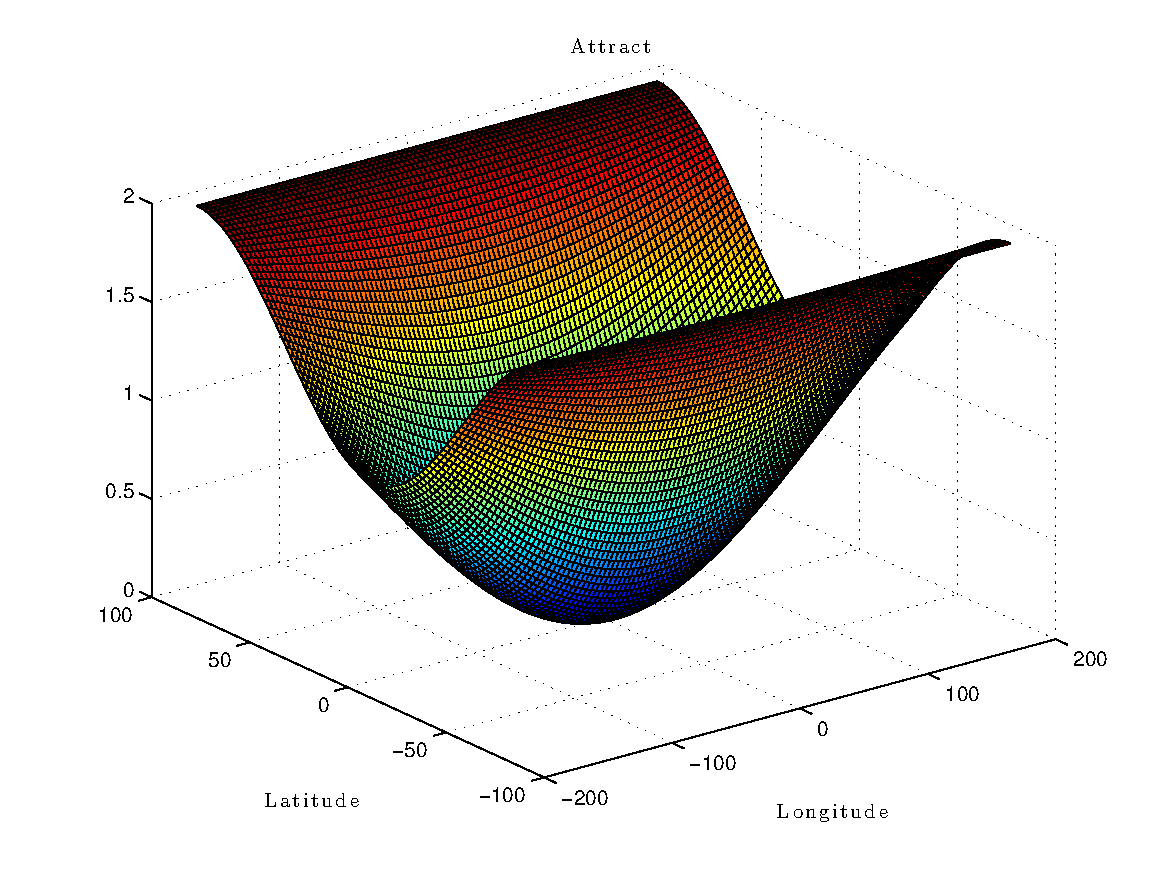
\includegraphics[width=\columnwidth]{attract_error} 
		\caption{Attractive \( A(R) \) } \label{fig:attract_error} 
	\end{subfigure}~ %add desired spacing between images, e. g. ~, \quad, \qquad, \hfill etc. %(or a blank line to force the subfigure onto a new line) 
	\begin{subfigure}[htbp]{0.33\columnwidth} 
		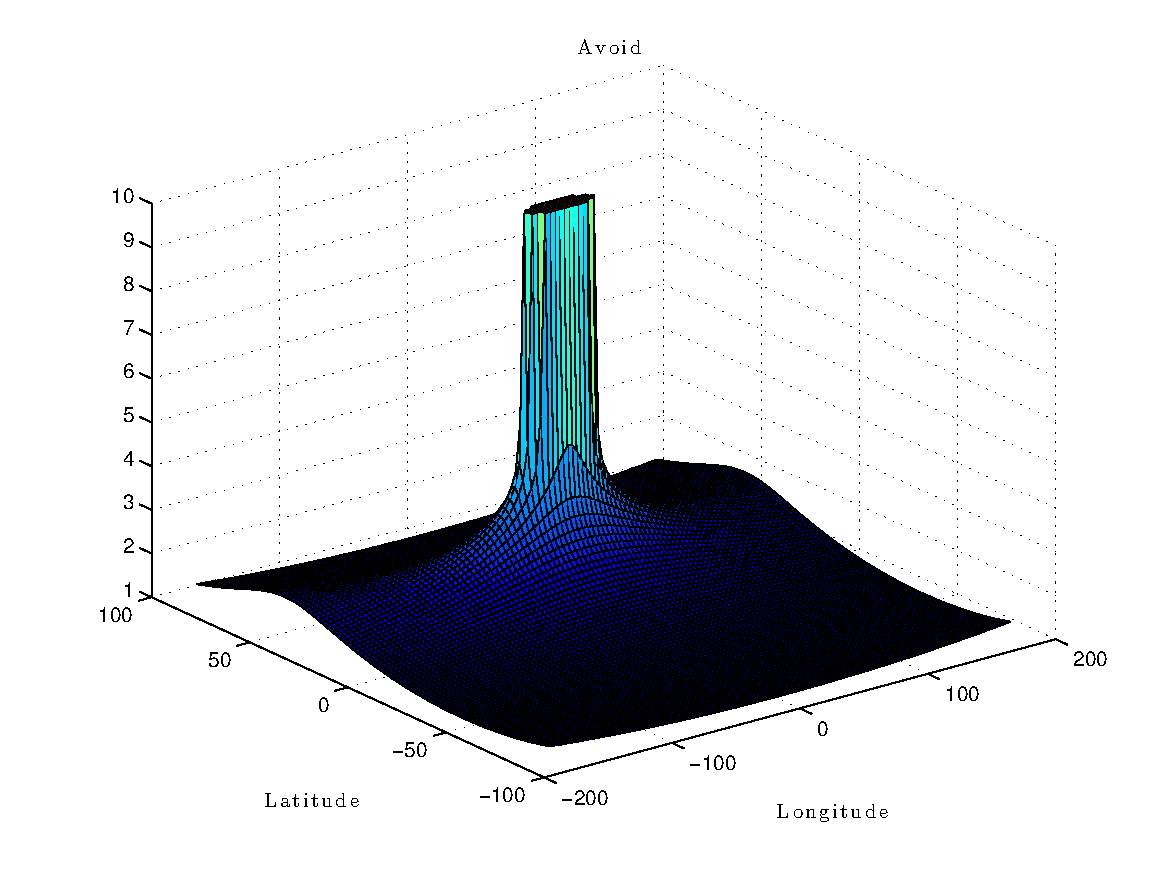
\includegraphics[width=\columnwidth]{avoid_error} 
		\caption{Repulsive \( B(R) \)} \label{fig:avoid_error} 
	\end{subfigure}~
	\begin{subfigure}[htbp]{0.33\columnwidth} 
		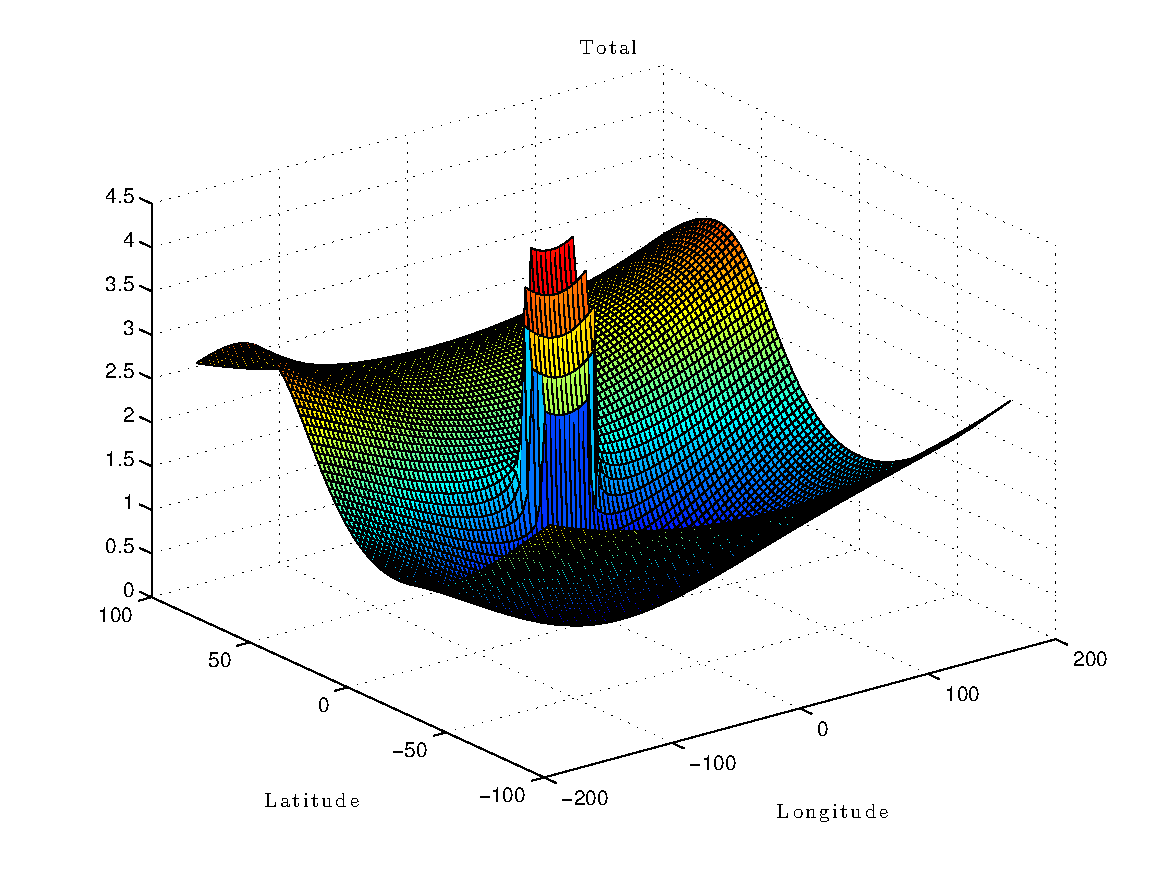
\includegraphics[width=\columnwidth]{combined_error} 
		\caption{Configuration \( \Psi \)} \label{fig:combined_error} 
	\end{subfigure}
	\caption{Configuration error function visualization}
	\label{fig:config_error} 
\end{figure}

\section{Results}\label{sec:results}
We demonstrate this new atttiude controller through numerical simulation and hardware experiment. 
A challenging attitude manuever is simulated to stabilize the system to a desired attitude. 
The control system automatically avoids four constrained regions, represented by the red cones in~\cref{fig:cad_adapt}, during the manuever.
The path of the body fixed sensor in the inertial frame, namely \( R r \), is illustrated in~\cref{fig:cad_adapt}.
The initial attitude is represented with the green circle while the final attitude is marked with a green \(\times\).
The control system is able to asymptotically converge to zero attitude error.
\begin{figure} 
	\centering 
	\begin{subfigure}[htbp]{0.45\columnwidth} 
		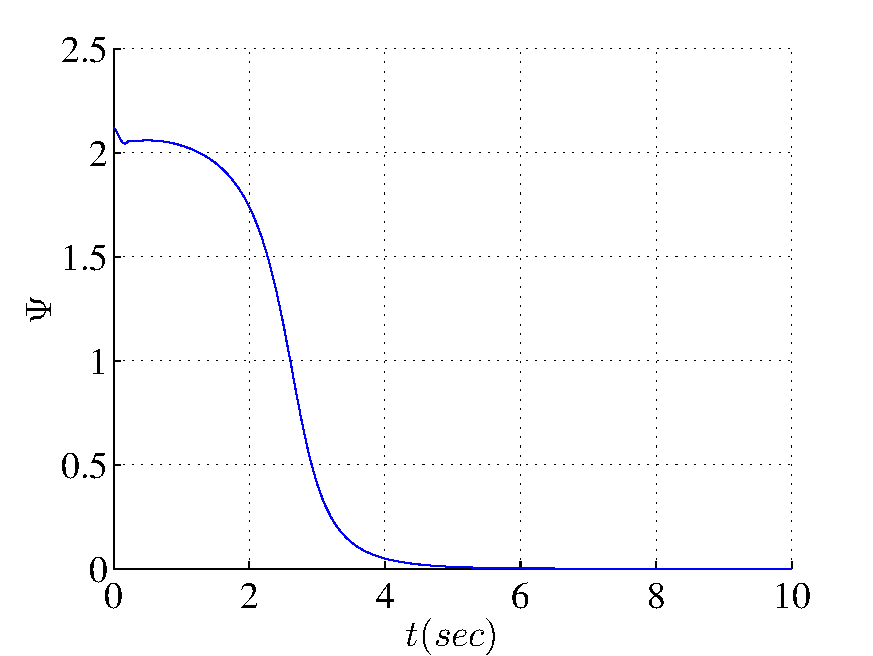
\includegraphics[width=\columnwidth]{Psi_adapt} 
		\caption{Configuration error \( \Psi \)} \label{fig:Psi_adapt} 
	\end{subfigure}~
	\begin{subfigure}[htbp]{0.45\columnwidth} 
		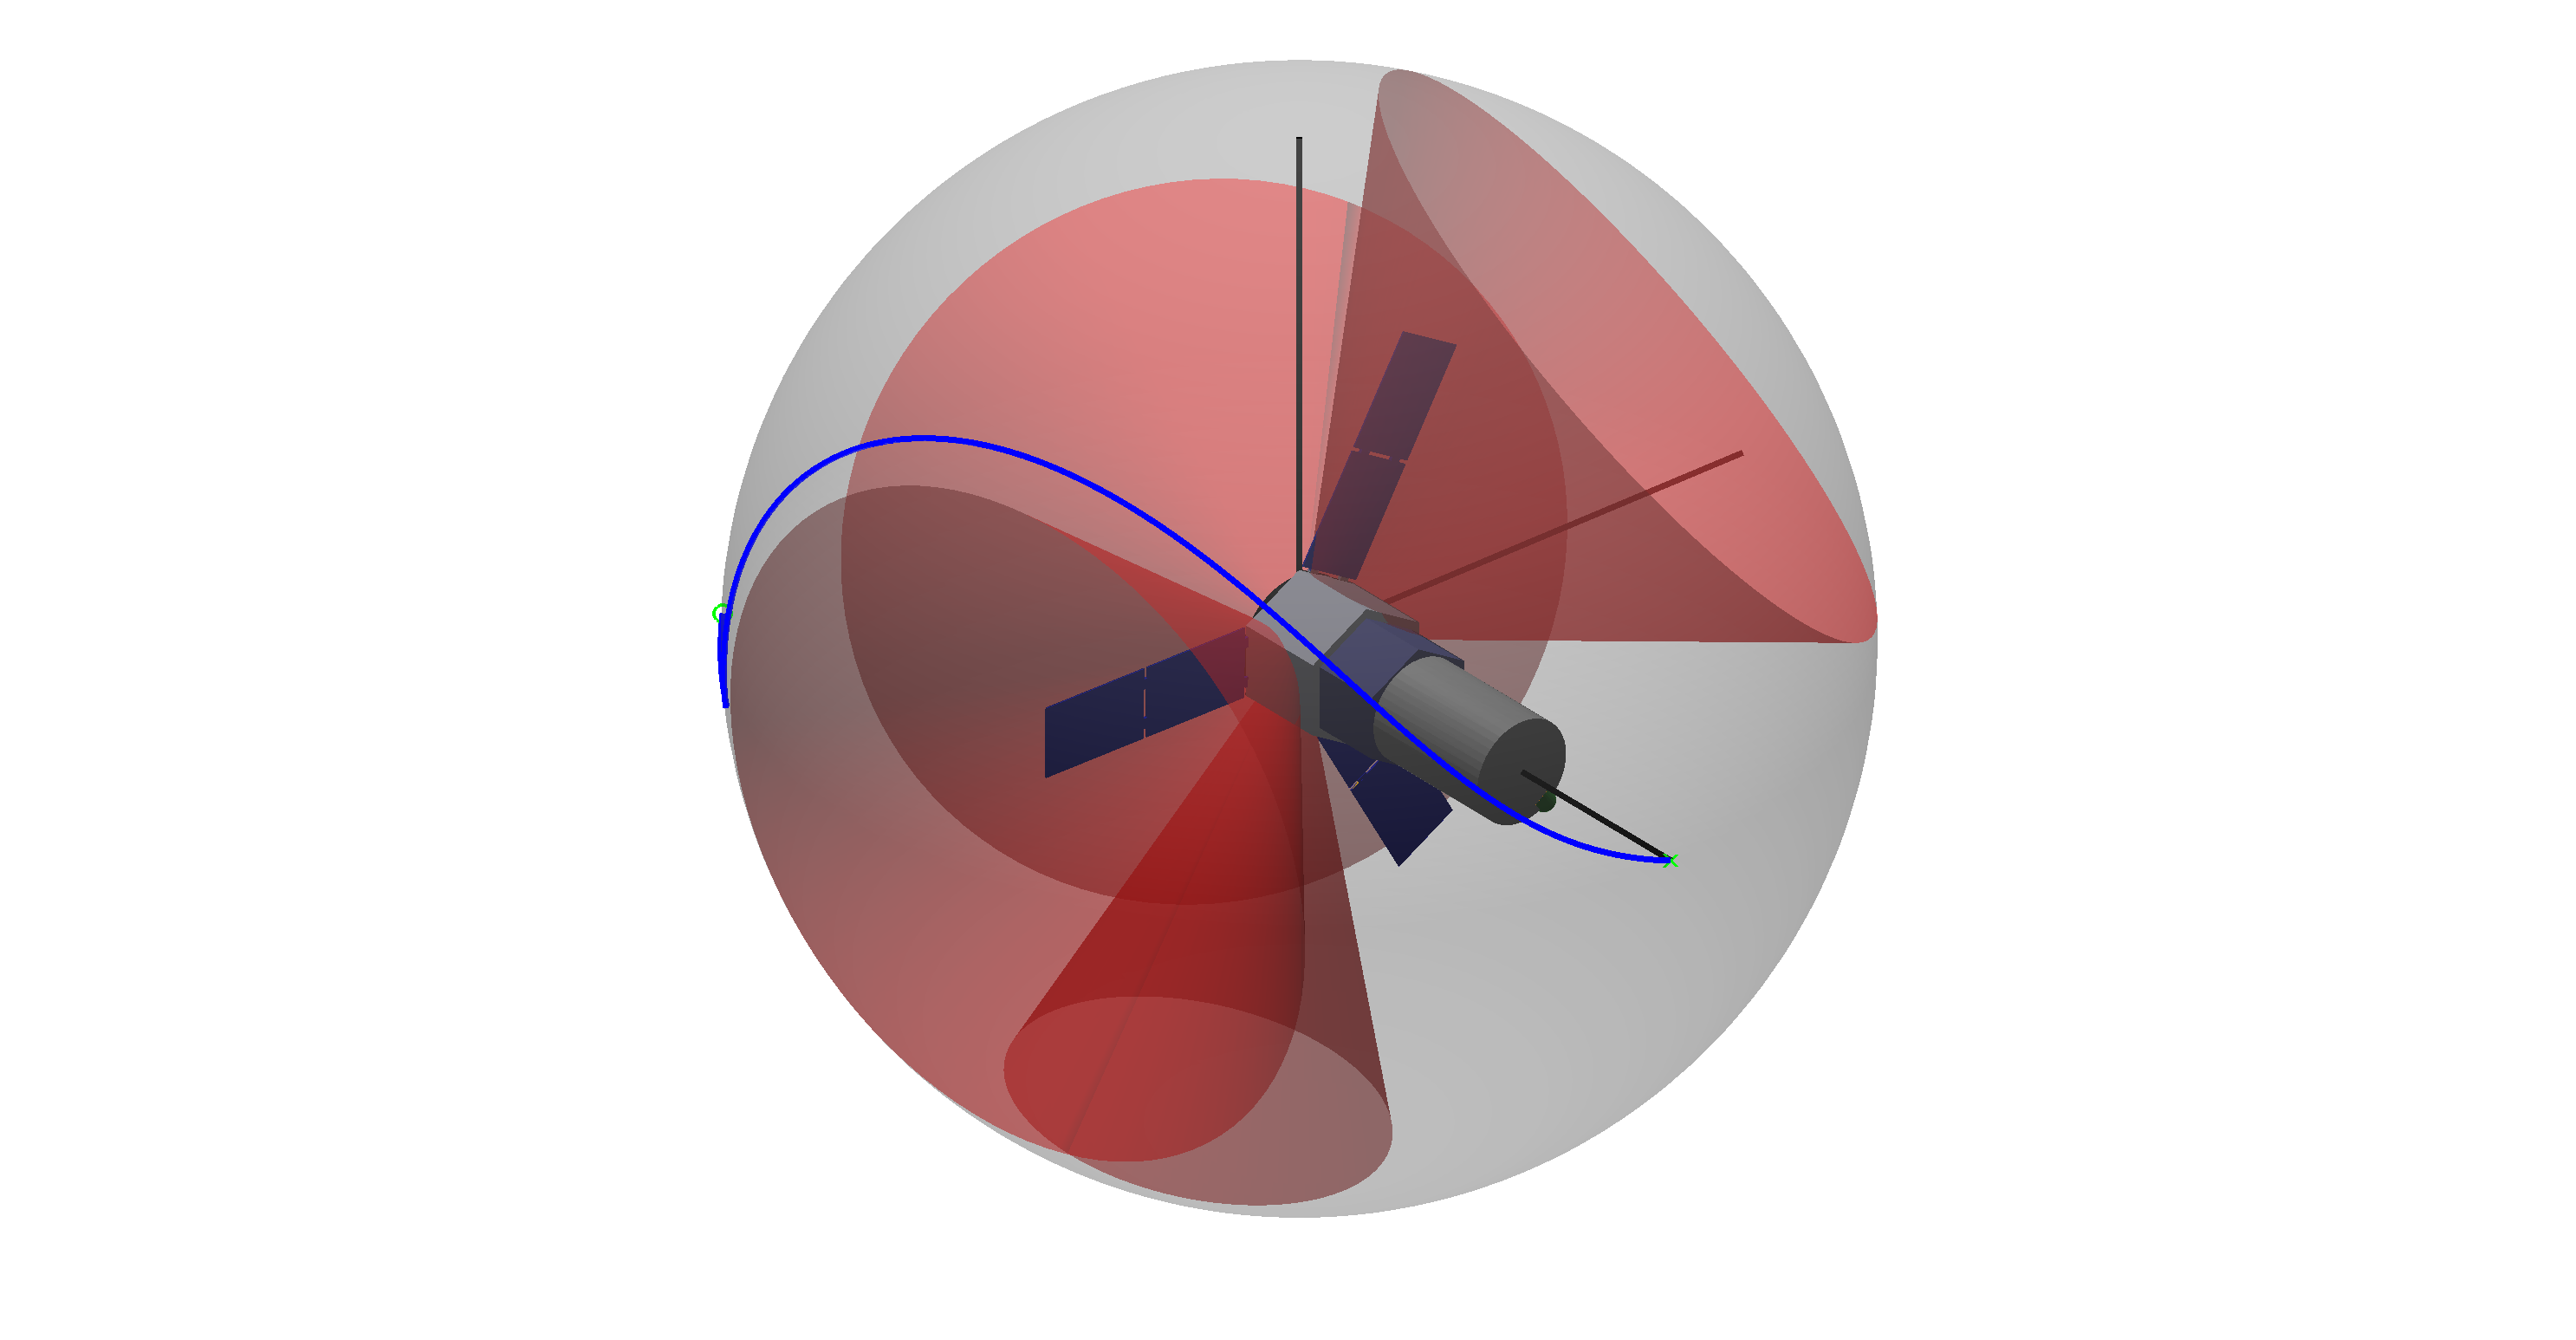
\includegraphics[trim=9cm 2.5cm 0 0,clip,width=1.29\columnwidth]{cad_adapt} 
		\caption{Attitude trajectory} \label{fig:cad_adapt} 
	\end{subfigure}
	\caption{Attitude stabilization simulation}
	\label{fig:adapt} 
\end{figure}
\subsection{Experiment}
We test the proposed control system on a UAV testbed.
A spherical joint is used to constrain the motion and test only the attitude dynamics.
A sensor pointing direction is defined in the body frame of the hexrotor and an obstacle in the inertial frame. 
An initial state is defined as \(R(0) = \exp( \frac{\pi}{2} \hat{e}_3) \), while the desired state is \(R_d =I \).
This results in the UAV performing a \ang{90} yaw rotation about the vertical axis of the spherical joint and the constrained region is on the shortest path connecting $R_0$ and $R_d$. 
\begin{figure} 
	\centering 
	\begin{subfigure}[htbp]{0.4\columnwidth} 
		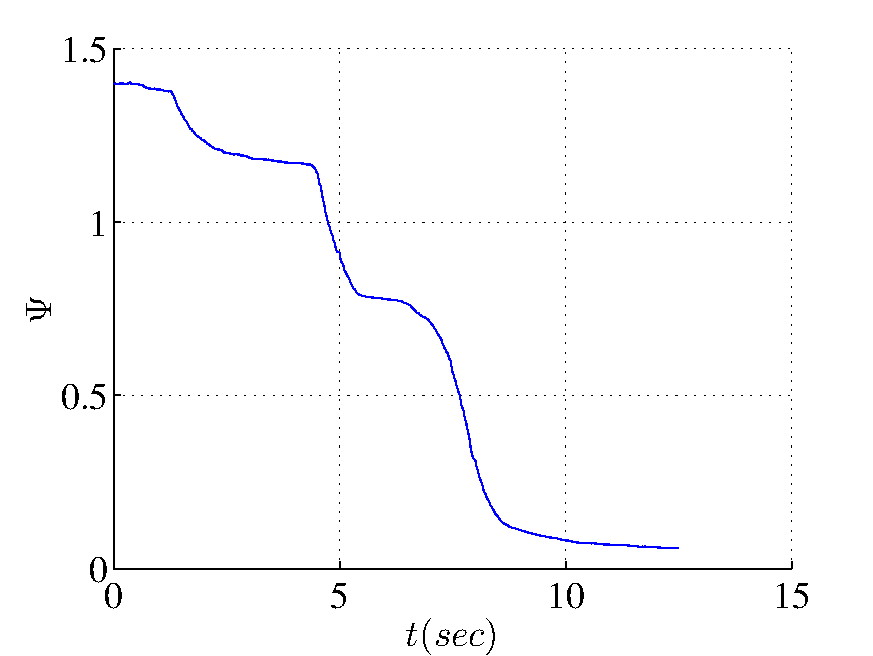
\includegraphics[width=\columnwidth]{Psi_exp} 
		\caption{Configuration error \( \Psi \)} \label{fig:Psi_exp} 
	\end{subfigure}~
	\begin{subfigure}[htbp]{0.4\columnwidth} 
		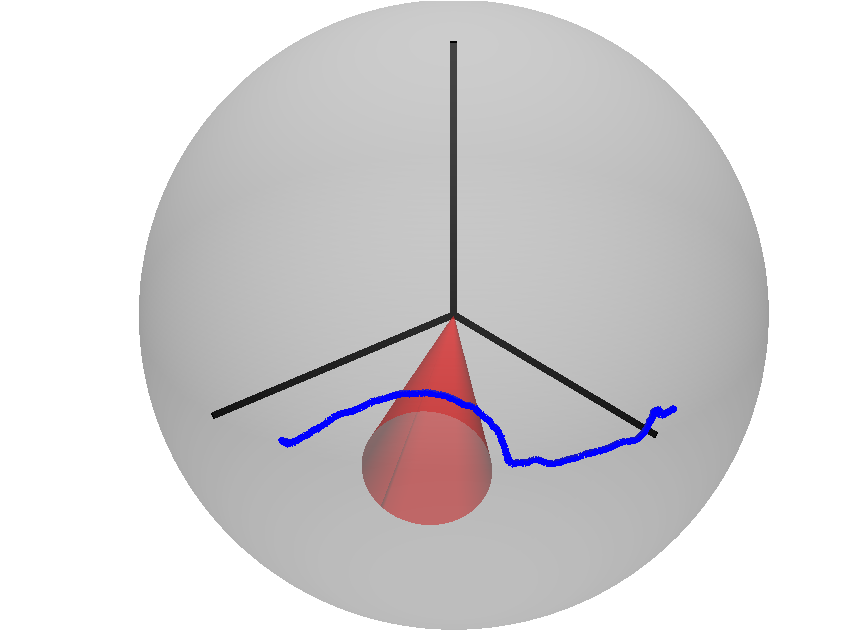
\includegraphics[width=\columnwidth]{traj_exp} 
		\caption{Attitude Trajectory} \label{fig:traj_exp} 
	\end{subfigure}
	\caption{Attitude stabilization experiment}
	\label{fig:exp} 
\end{figure}

The experimental results are shown in~\Cref{fig:exp}.
The attitude error asymptotically converges to zero. 
The hexrotor avoids the constrained region illustrated by the circular cone in~\cref{fig:traj_exp}, by rotating around the boundary of the constraint. 
This verifies that the proposed control system exhibits the desired performance in the experimental setting. 
A video clip showing the attitude manuever is available at \url{https://youtu.be/dsmAbwQram4}.
\section{Conclusions}\label{sec:conclusions}
We have developed a geometric adaptive control system which incorporates state inequality constraints on \(\SO\) for the first time.
The presented control system is developed directly on \(\SO\) and it avoids singularities and ambiguities that are inherent to attitude parameterizations.
We have demonstrated the control system via numerical simulation and hardware experiments on a hexrotor UAV.
Compared to the previous work on constrained attitude control, we present a geometrically exact control system without parameterizations.
This is in contrast to many state constrained attitude control systems which require an a priori attitude trajectory to be calculated. 
The presented method is simple, efficient and ideal for hardware implementation on embedded systems.

%%%%%%%%%%%%%%%%%%%%%%%%%%%%%%%%%%%%%%%%%%%%%%%%%%%%%%%%%%%%%%%%%%%%%%%%%%%%%%%%

%\addtolength{\textheight}{-12cm}   % This command serves to balance the column lengths
                                  % on the last page of the document manually. It shortens
                                  % the textheight of the last page by a suitable amount.
                                  % This command does not take effect until the next page
                                  % so it should come on the page before the last. Make
                                  % sure that you do not shorten the textheight too much.
                                  
\bibliography{library}
\bibliographystyle{IEEEtran}

\end{document}
